\documentclass[10pt]{article}

\usepackage[a3paper, landscape, margin=0.8cm, top=0.7cm, bottom=0.7cm]{geometry}
\usepackage[utf8]{inputenc}
\usepackage[T1]{fontenc}
\usepackage{lmodern}
\usepackage{graphicx}
\usepackage[table]{xcolor}
\usepackage{amsmath,amssymb}
\usepackage{booktabs}
\usepackage{tabularx}
\usepackage{microtype}
\usepackage{tikz}
\usetikzlibrary{calc,positioning}

\graphicspath{{../outputs/figures/}{outputs/figures/}}

% Executive Showcase Color Palette
\definecolor{headerblue}{RGB}{18, 43, 76}       % Deep Navy
\definecolor{accentgold}{RGB}{212, 160, 23}      % Warm Gold
\definecolor{cardbg}{RGB}{250, 252, 255}         % Crisp Light Slate
\definecolor{cardborder}{RGB}{203, 213, 225}     % Slate Border
\definecolor{kpibg}{RGB}{241, 245, 249}          % Light Gray
\definecolor{kpicard}{RGB}{255, 255, 255}        % White Tile
\definecolor{highlightbg}{RGB}{236, 253, 245}    % Soft Mint Green
\definecolor{highlightborder}{RGB}{16, 185, 129} % Emerald Green
\definecolor{alertred}{RGB}{185, 28, 28}         % Crimson Red

\pagestyle{empty}
\setlength{\parindent}{0pt}
\setlength{\parskip}{0pt}

\newcommand{\INR}{\text{INR~}}
\newcommand{\Rs}{\text{Rs.~}}

\begin{document}

% ----------------------------------------------------------------------------
% HEADER BLOCK
% ----------------------------------------------------------------------------
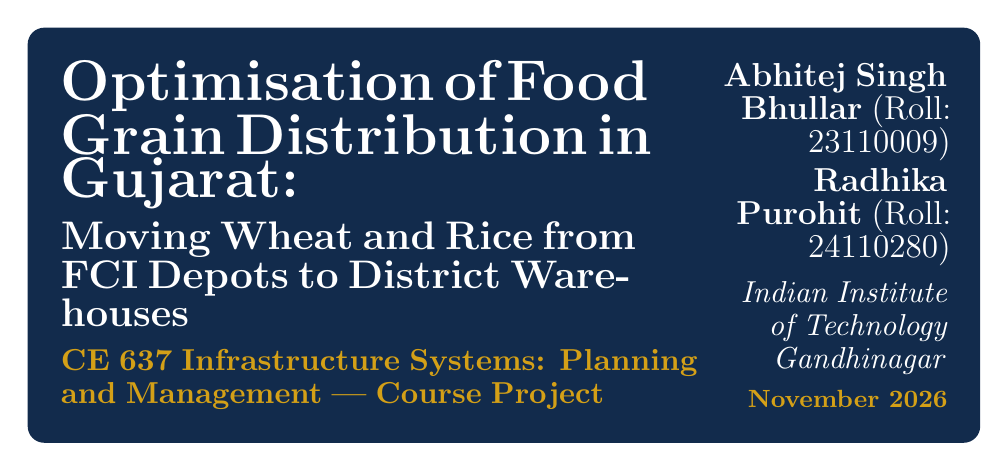
\begin{tikzpicture}
  \node[fill=headerblue, rounded corners=6pt, inner sep=12pt, text width=\linewidth-24.8pt] {
    \begin{minipage}[c]{0.72\linewidth}
      \color{white}
      {\fontsize{22pt}{26pt}\selectfont \textbf{Optimisation of Food Grain Distribution in Gujarat:}}\\[4pt]
      {\fontsize{15pt}{18pt}\selectfont \textbf{Moving Wheat and Rice from FCI Depots to District Warehouses}}\\[4pt]
      {\fontsize{11pt}{13pt}\selectfont \textbf{\color{accentgold}CE 637 Infrastructure Systems: Planning and Management --- Course Project}}
    \end{minipage}\hfill
    \begin{minipage}[c]{0.26\linewidth}
      \color{white}\raggedleft
      {\fontsize{12pt}{15pt}\selectfont \textbf{Abhitej Singh Bhullar} (Roll: 23110009)}\\[2pt]
      {\fontsize{12pt}{15pt}\selectfont \textbf{Radhika Purohit} (Roll: 24110280)}\\[4pt]
      {\fontsize{10.5pt}{13pt}\selectfont \textit{Indian Institute of Technology Gandhinagar}}\\[2pt]
      {\fontsize{9.5pt}{12pt}\selectfont \textcolor{accentgold}{\textbf{November 2026}}}
    \end{minipage}
  };
\end{tikzpicture}

\vspace{0.3cm}

% ----------------------------------------------------------------------------
% TWO-COLUMN BODY LAYOUT
% ----------------------------------------------------------------------------
\begin{minipage}[t]{0.485\linewidth}\vspace{0pt}

  % ==========================================================================
  % SECTION 1: THE QUESTION & SYSTEM TOPOLOGY
  % ==========================================================================
  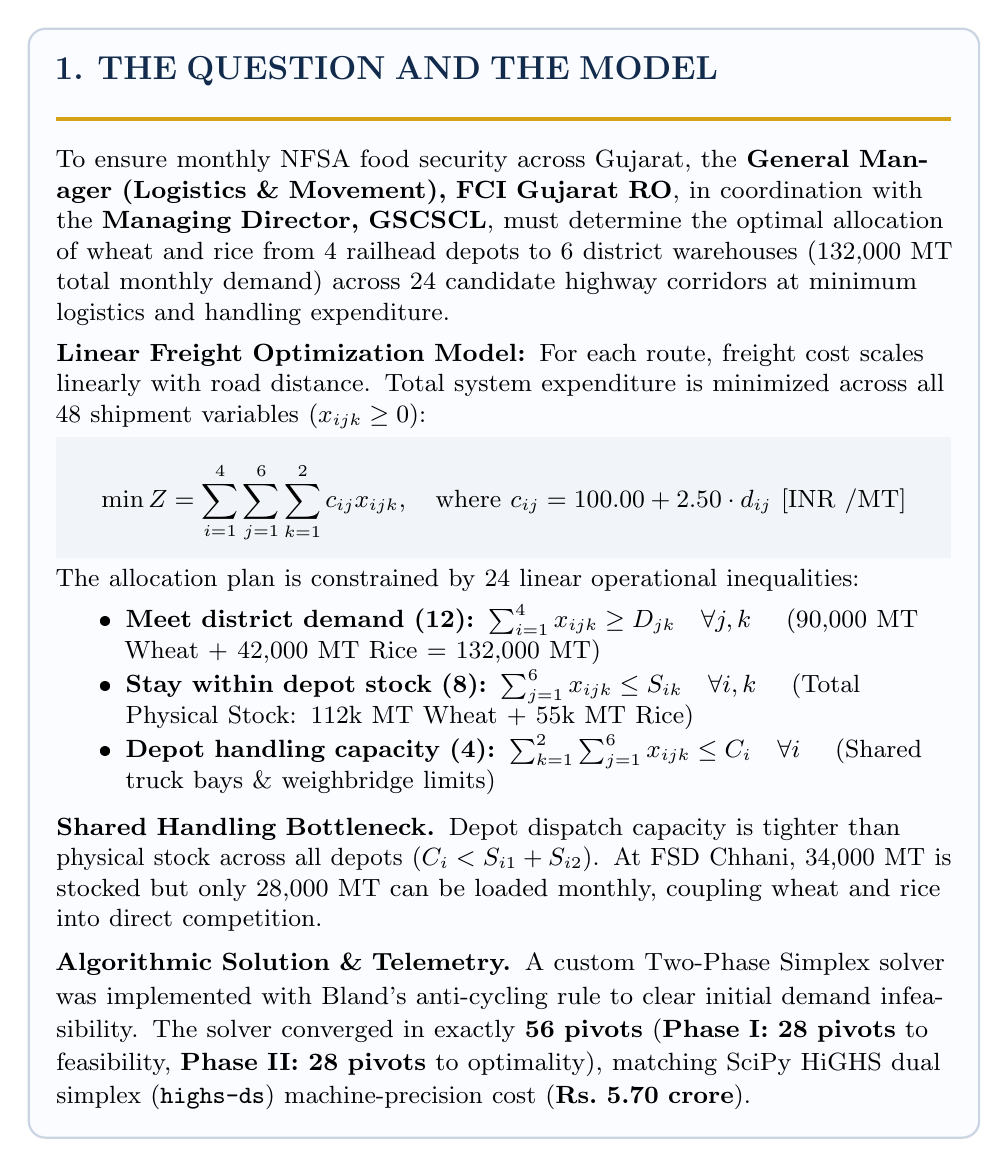
\begin{tikzpicture}
    \node[draw=cardborder, fill=cardbg, rounded corners=6pt, line width=0.8pt, inner sep=10pt, text width=\linewidth-21.6pt] {
      {\fontsize{13pt}{15pt}\selectfont \textbf{\color{headerblue}1. THE QUESTION AND THE MODEL}}\\[3pt]
      {\color{accentgold}\rule{\linewidth}{1.2pt}}\\[6pt]
      \small

      To ensure monthly NFSA food security across Gujarat, the \textbf{General Manager (Logistics \& Movement), FCI Gujarat RO}, in coordination with the \textbf{Managing Director, GSCSCL}, must determine the optimal allocation of wheat and rice from 4 railhead depots to 6 district warehouses (132,000 MT total monthly demand) across 24 candidate highway corridors at minimum logistics and handling expenditure.\\[4pt]
      \textbf{Linear Freight Optimization Model:} For each route, freight cost scales linearly with road distance. Total system expenditure is minimized across all 48 shipment variables ($x_{ijk} \ge 0$):\par\vspace{2pt}
      \noindent\colorbox{kpibg}{\parbox{\dimexpr\linewidth-2\fboxsep\relax}{
        \vspace{-3pt}
        \[
          \min Z = \sum_{i=1}^4 \sum_{j=1}^6 \sum_{k=1}^2 c_{ij} x_{ijk}, \quad \text{where } c_{ij} = 100.00 + 2.50 \cdot d_{ij} \text{ [\INR/MT]}
        \]
        \vspace{-7pt}
      }}\par\vspace{3pt}
      The allocation plan is constrained by 24 linear operational inequalities:
      \begin{itemize}\setlength{\itemsep}{1.5pt}\setlength{\parskip}{0pt}\small
        \item \textbf{Meet district demand (12):} $\sum_{i=1}^4 x_{ijk} \ge D_{jk} \quad \forall j, k$ \quad (90,000 MT Wheat + 42,000 MT Rice = 132,000 MT)
        \item \textbf{Stay within depot stock (8):} $\sum_{j=1}^6 x_{ijk} \le S_{ik} \quad \forall i, k$ \quad (Total Physical Stock: 112k MT Wheat + 55k MT Rice)
        \item \textbf{Depot handling capacity (4):} $\sum_{k=1}^2 \sum_{j=1}^6 x_{ijk} \le C_i \quad \forall i$ \quad (Shared truck bays \& weighbridge limits)
      \end{itemize}
      \vspace{2pt}

      \textbf{Shared Handling Bottleneck.} Depot dispatch capacity is tighter than physical stock across all depots ($C_i < S_{i1} + S_{i2}$). At FSD Chhani, 34,000 MT is stocked but only 28,000 MT can be loaded monthly, coupling wheat and rice into direct competition.\\[4pt]
      \textbf{Algorithmic Solution \& Telemetry.} A custom Two-Phase Simplex solver was implemented with Bland's anti-cycling rule to clear initial demand infeasibility. The solver converged in exactly \textbf{56 pivots} (\textbf{Phase I: 28 pivots} to feasibility, \textbf{Phase II: 28 pivots} to optimality), matching SciPy HiGHS dual simplex (\texttt{highs-ds}) machine-precision cost (\textbf{\Rs 5.70 crore}).
    };
  \end{tikzpicture}

  \vspace{0.35cm}

  % ==========================================================================
  % SECTION 2: THE RECOMMENDED ANSWER & SURAT BOTTLENECK
  % ==========================================================================
  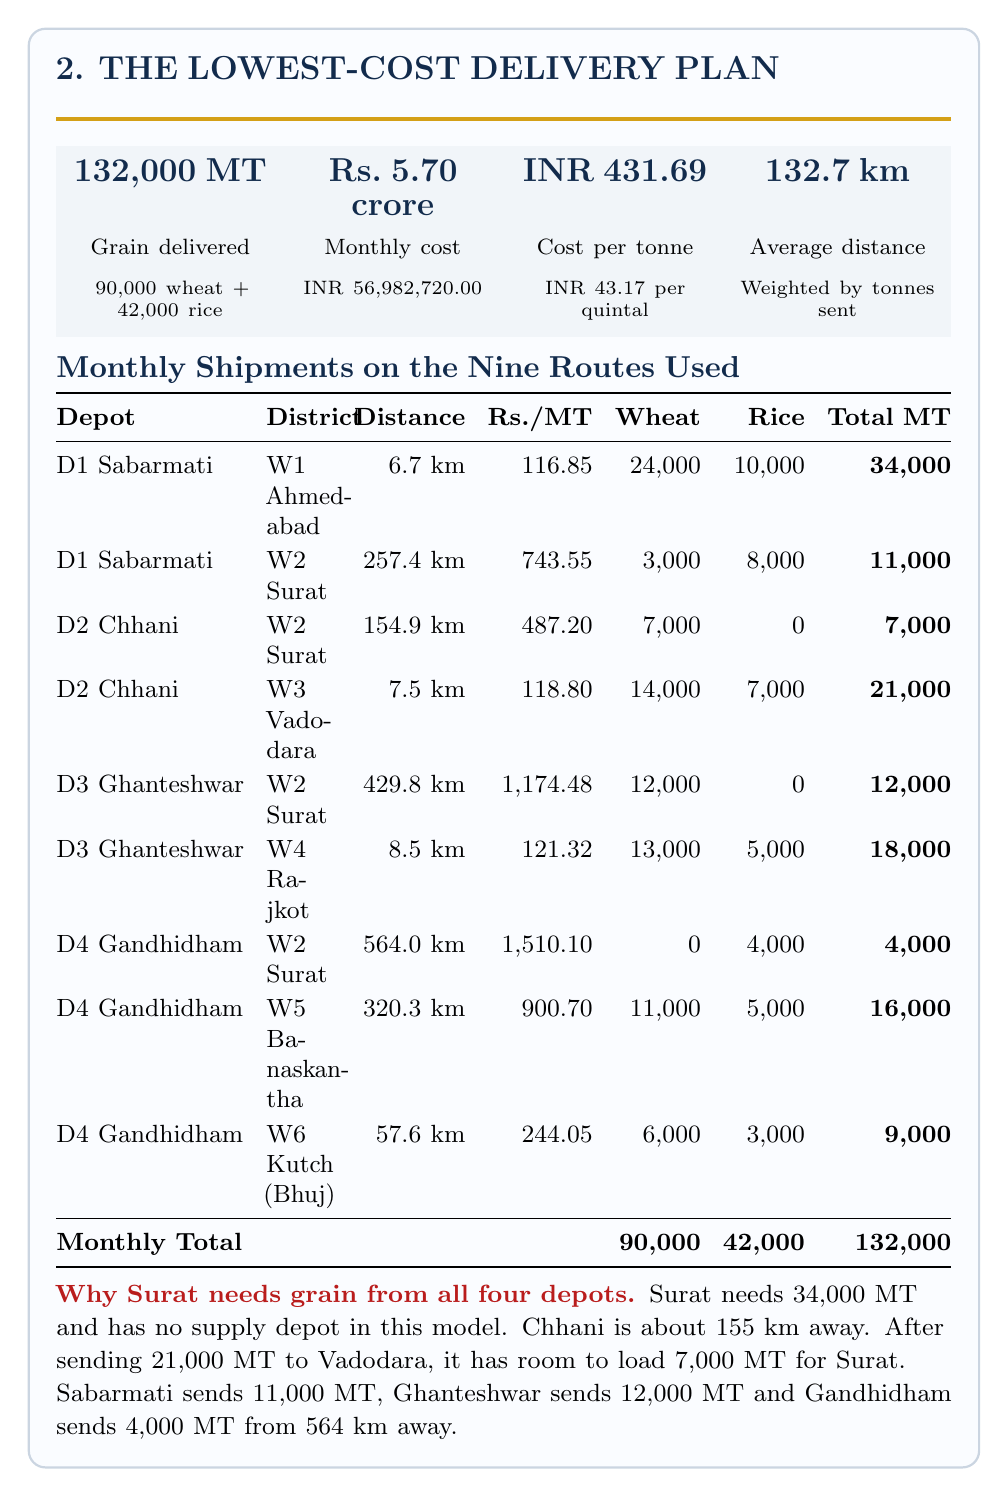
\begin{tikzpicture}
    \node[draw=cardborder, fill=cardbg, rounded corners=6pt, line width=0.8pt, inner sep=10pt, text width=\linewidth-21.6pt] {
      {\fontsize{13pt}{15pt}\selectfont \textbf{\color{headerblue}2. THE LOWEST-COST DELIVERY PLAN}}\\[3pt]
      {\color{accentgold}\rule{\linewidth}{1.2pt}}\\[6pt]
      
      % KPI Banner Tiles
      \vspace{2pt}
      \noindent\colorbox{kpibg}{\parbox{\dimexpr\linewidth-2\fboxsep\relax}{
        \renewcommand{\arraystretch}{1.2}
        \setlength{\tabcolsep}{2pt}

        \begin{tabularx}{\linewidth}{@{}*{4}{>{\centering\arraybackslash}X}@{}}
          \textbf{\large\color{headerblue}132,000 MT} &
          \textbf{\large\color{headerblue}\Rs 5.70 crore} &
          \textbf{\large\color{headerblue}\INR 431.69} &
          \textbf{\large\color{headerblue}132.7 km} \\
          \footnotesize Grain delivered &
          \footnotesize Monthly cost &
          \footnotesize Cost per tonne &
          \footnotesize Average distance \\
          \scriptsize 90,000 wheat + 42,000 rice &
          \scriptsize \INR 56,982,720.00 &
          \scriptsize \INR 43.17 per quintal &
          \scriptsize Weighted by tonnes sent \\
        \end{tabularx}
      }}
      
      \vspace{6pt}
      {\fontsize{10.5pt}{13pt}\selectfont \textbf{\color{headerblue}Monthly Shipments on the Nine Routes Used}}\\[2pt]
      \centering
      \small
      \renewcommand{\arraystretch}{1.12}
      \setlength{\tabcolsep}{4pt}
      \begin{tabularx}{\linewidth}{@{}lXr>{\raggedleft\arraybackslash}r>{\raggedleft\arraybackslash}r>{\raggedleft\arraybackslash}r>{\raggedleft\arraybackslash}r@{}}
        \toprule
        \textbf{Depot} & \textbf{District} & \textbf{Distance} & \textbf{Rs./MT} & \textbf{Wheat} & \textbf{Rice} & \textbf{Total MT} \\
        \midrule
        D1 Sabarmati & W1 Ahmedabad & 6.7 km & 116.85 & 24,000 & 10,000 & \textbf{34,000} \\
        D1 Sabarmati & W2 Surat & 257.4 km & 743.55 & 3,000 & 8,000 & \textbf{11,000} \\
        D2 Chhani & W2 Surat & 154.9 km & 487.20 & 7,000 & 0 & \textbf{7,000} \\
        D2 Chhani & W3 Vadodara & 7.5 km & 118.80 & 14,000 & 7,000 & \textbf{21,000} \\
        D3 Ghanteshwar & W2 Surat & 429.8 km & 1,174.48 & 12,000 & 0 & \textbf{12,000} \\
        D3 Ghanteshwar & W4 Rajkot & 8.5 km & 121.32 & 13,000 & 5,000 & \textbf{18,000} \\
        D4 Gandhidham & W2 Surat & 564.0 km & 1,510.10 & 0 & 4,000 & \textbf{4,000} \\
        D4 Gandhidham & W5 Banaskantha & 320.3 km & 900.70 & 11,000 & 5,000 & \textbf{16,000} \\
        D4 Gandhidham & W6 Kutch (Bhuj) & 57.6 km & 244.05 & 6,000 & 3,000 & \textbf{9,000} \\
        \midrule
        \multicolumn{4}{@{}l}{\textbf{Monthly Total}} & \textbf{90,000} & \textbf{42,000} & \textbf{132,000} \\
        \bottomrule
      \end{tabularx}

      \vspace{5pt}
      \raggedright \small

      \textbf{\color{alertred}Why Surat needs grain from all four depots.}
      Surat needs 34,000 MT and has no supply depot in this model. Chhani is about 155 km away. After sending 21,000 MT to Vadodara, it has room to load 7,000 MT for Surat. Sabarmati sends 11,000 MT, Ghanteshwar sends 12,000 MT and Gandhidham sends 4,000 MT from 564 km away.
    };
  \end{tikzpicture}

\end{minipage}\hfill
\begin{minipage}[t]{0.495\linewidth}\vspace{0pt}

  % ==========================================================================
  % SECTION 3: KEY FIGURE — OPTIMAL NETWORK FLOW MAP
  % ==========================================================================
  \begin{tikzpicture}
    \node[draw=cardborder, fill=cardbg, rounded corners=6pt, line width=0.8pt, inner sep=10pt, text width=\linewidth-21.6pt] {
      {\fontsize{13pt}{15pt}\selectfont \textbf{\color{headerblue}3. WHERE THE GRAIN GOES}}\\[3pt]
      {\color{accentgold}\rule{\linewidth}{1.2pt}}\\[6pt]
      \centering
      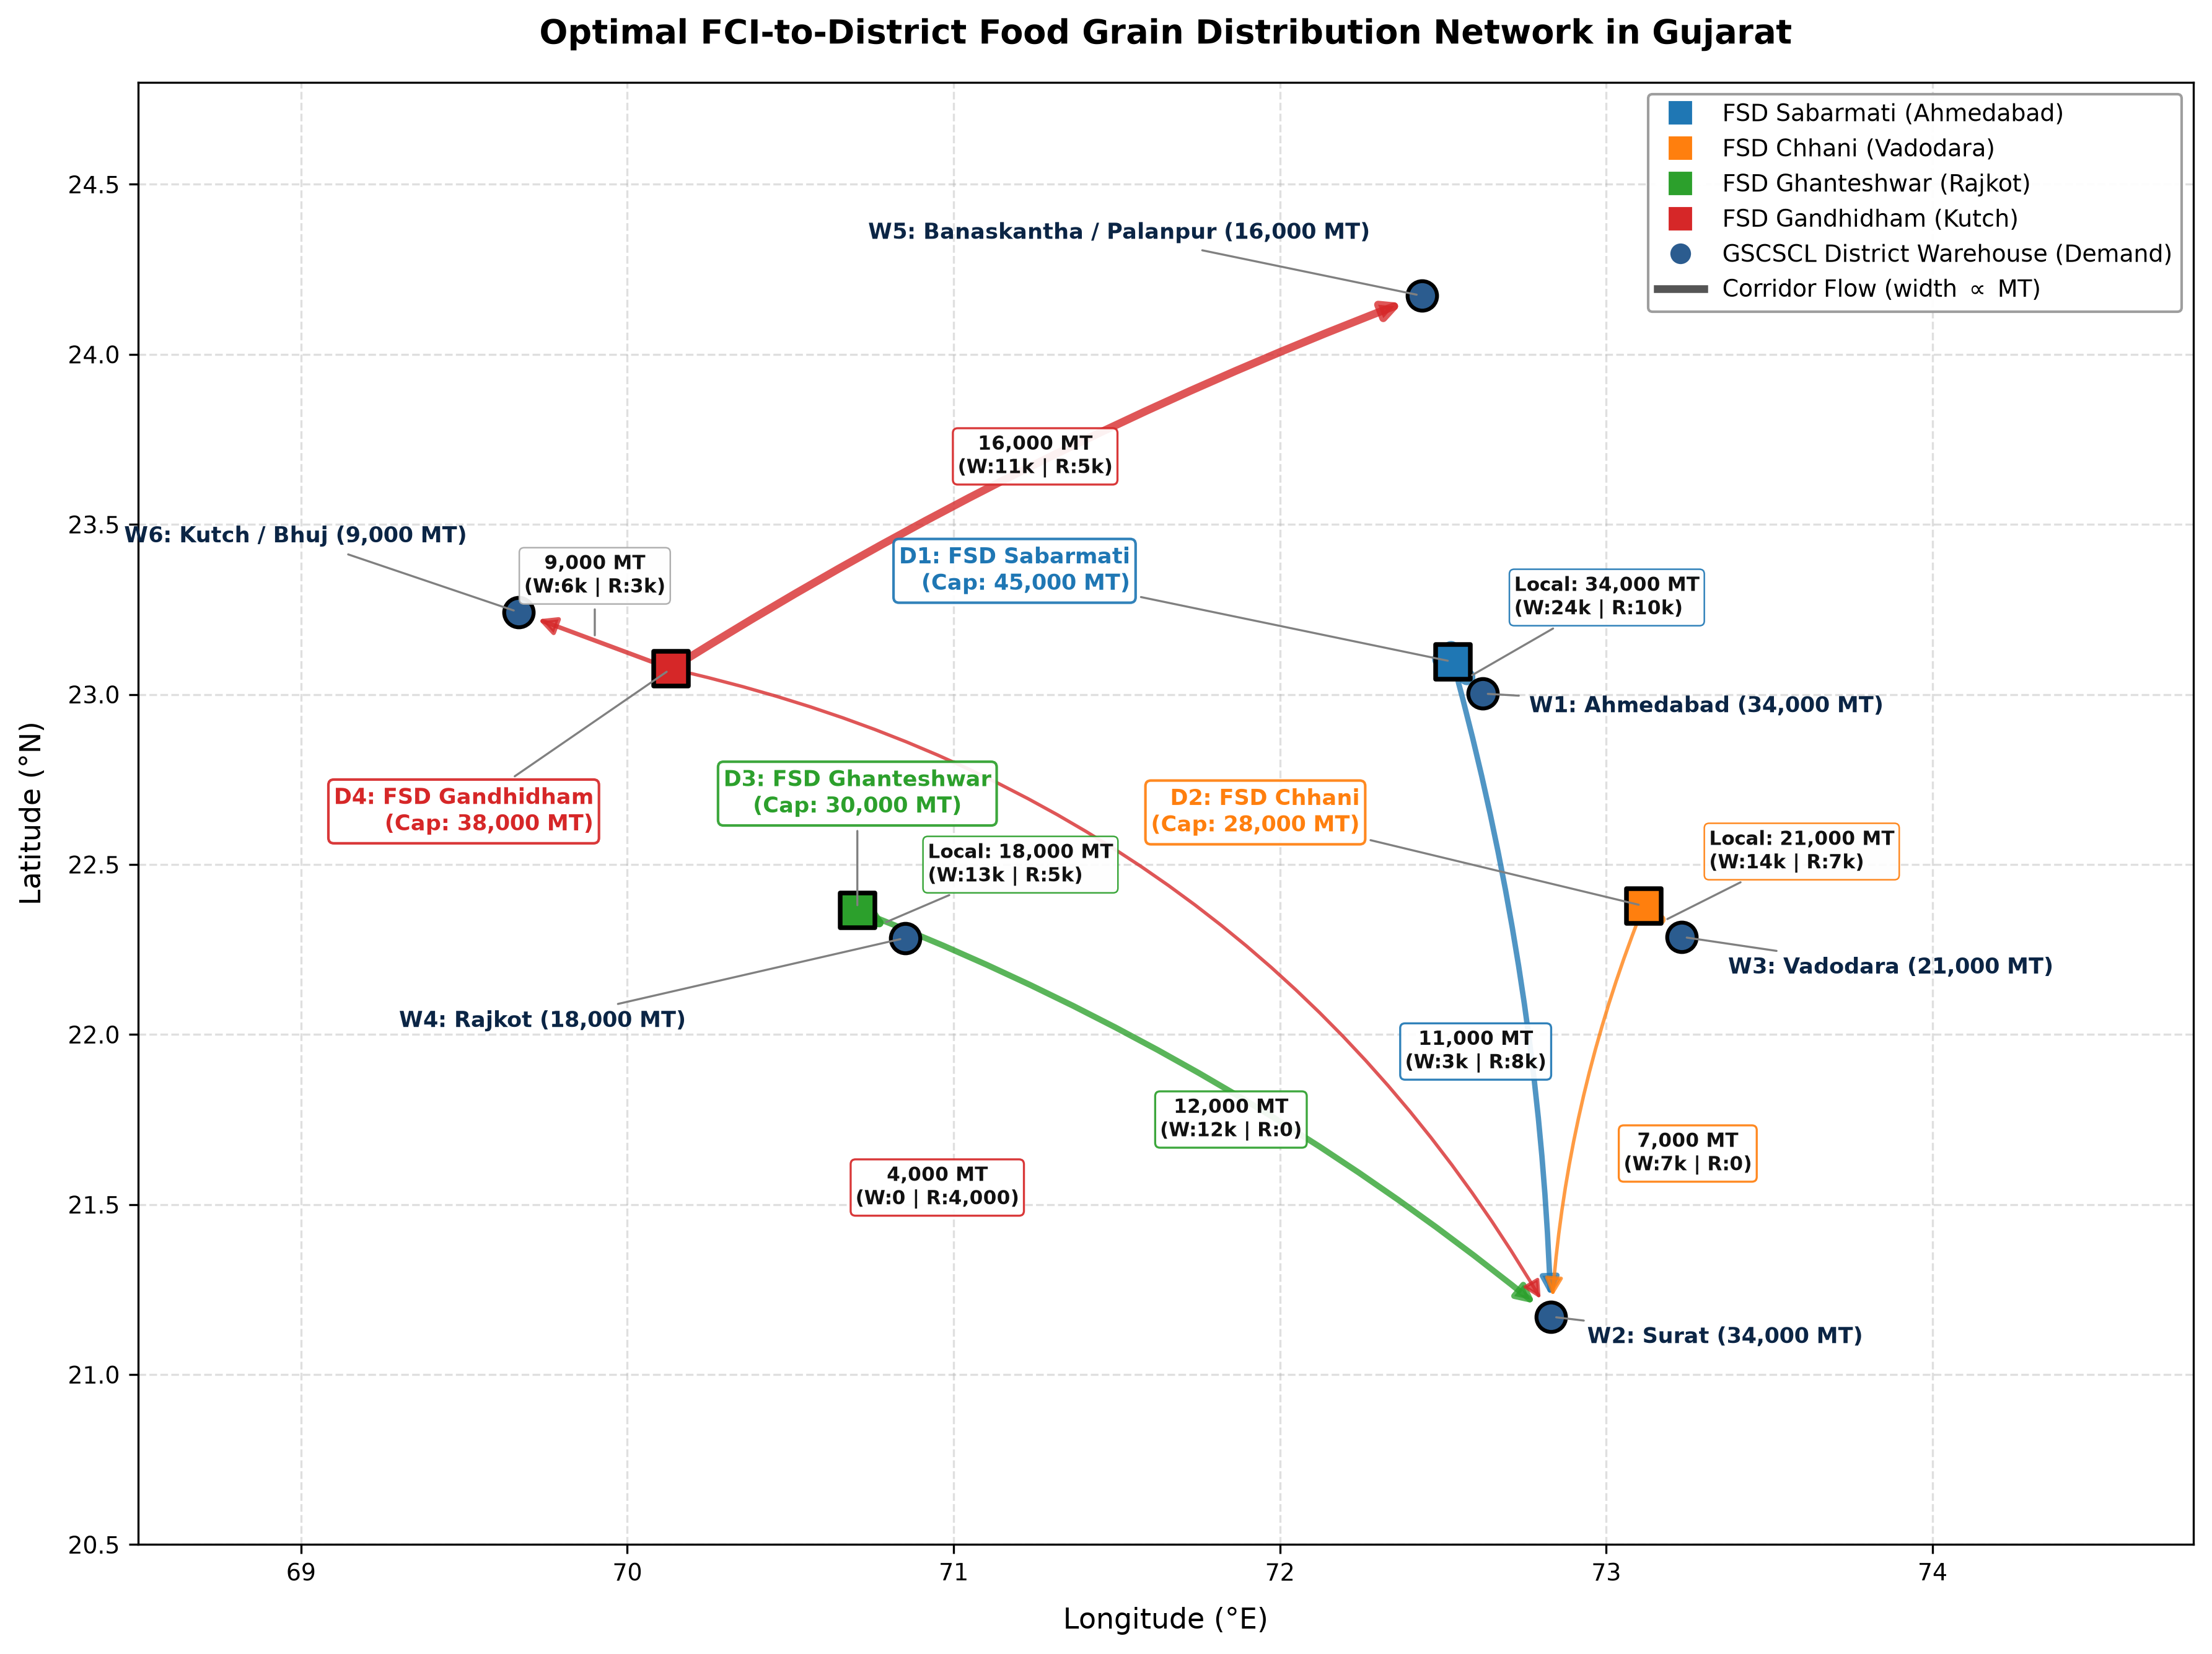
\includegraphics[width=0.97\linewidth, height=9.6cm, keepaspectratio]{fig1_network_flow_map.png}\\[4pt]
      \raggedright \small

      The lowest-cost plan uses nine of the 24 routes. Ahmedabad, Vadodara, Rajkot and Bhuj each receive their grain from a nearby depot. Surat receives grain from all four. The lines show which depots serve which districts. Thicker lines carry more grain.
    };
  \end{tikzpicture}

  \vspace{0.35cm}

  % ==========================================================================
  % SECTION 4: SENSITIVITY & BOTTLENECK INSIGHT
  % ==========================================================================
  \begin{tikzpicture}
    \node[draw=cardborder, fill=cardbg, rounded corners=6pt, line width=0.8pt, inner sep=10pt, text width=\linewidth-21.6pt] {
      {\fontsize{13pt}{15pt}\selectfont \textbf{\color{headerblue}4. WHAT IF CHHANI COULD LOAD MORE?}}\\[3pt]
      {\color{accentgold}\rule{\linewidth}{1.2pt}}\\[6pt]
      
      \begin{minipage}[t]{0.46\linewidth}\vspace{0pt}
        \centering
        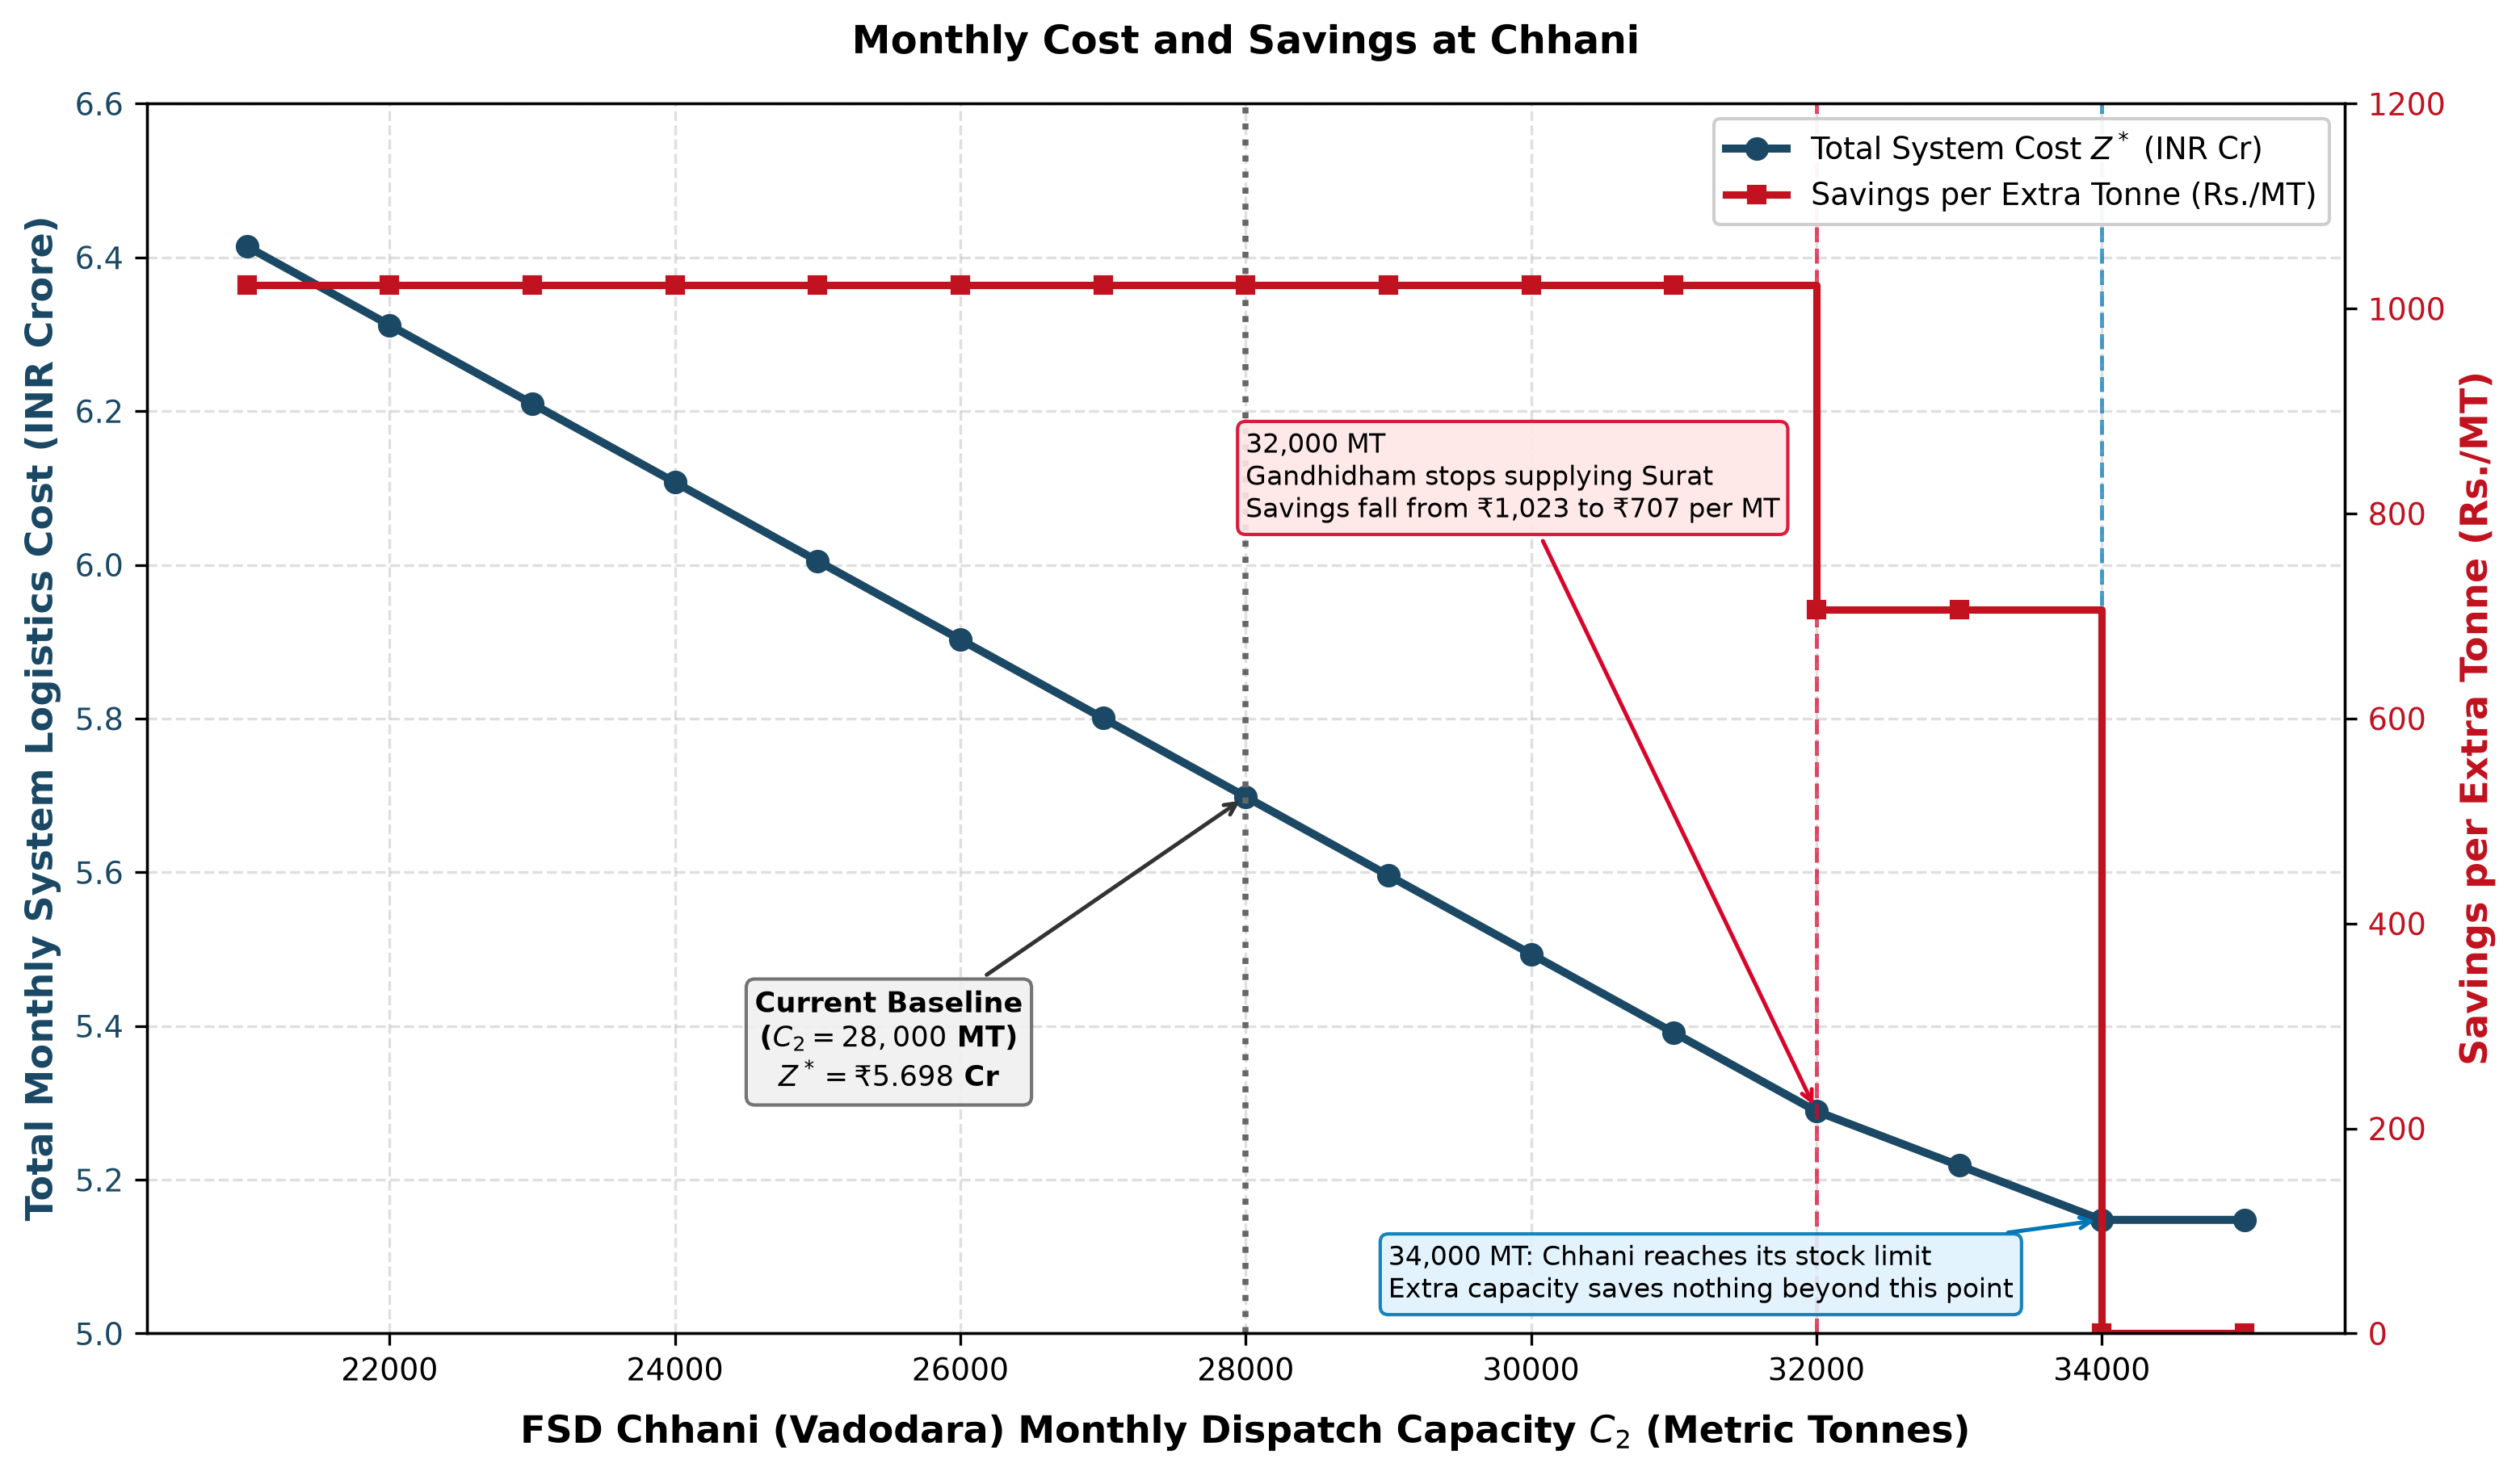
\includegraphics[width=\linewidth, height=6.6cm, keepaspectratio]{fig3_sensitivity_curve.png}\\[2pt]
        {\footnotesize Monthly cost and savings from adding loading capacity at Chhani.}
      \end{minipage}\hfill
      \begin{minipage}[t]{0.51\linewidth}\vspace{0pt}
        \raggedright \small

        \textbf{\color{headerblue}Two steps to lower monthly costs}
        \begin{itemize}\setlength{\itemsep}{3pt}\setlength{\parskip}{0pt}\small
          \item \textbf{Step 1 (28,000 to 32,000 MT).}
          Chhani replaces Gandhidham's shipments to Surat. Each tonne saves Rs.~1,510.10 minus Rs.~487.20, or \textbf{Rs.~1,022.90}. Over 4,000 MT, that saves \textbf{Rs.~40,91,600}.
          \item \textbf{Step 2 (32,000 to 34,000 MT).}
          Chhani takes over more of Surat's demand from Sabarmati, which can then replace Gandhidham in Banaskantha. The two changes save Rs.~256.35 and Rs.~450.20 per tonne, or \textbf{Rs.~706.55} together. Over 2,000 MT, that saves \textbf{Rs.~14,13,100}.
          \item Beyond 34,000 MT, more loading capacity saves nothing because Chhani has no more grain to send.
        \end{itemize}
      \end{minipage}

      \vspace{6pt}
      % High-Impact Actionable Policy Callout Box
      \begin{tikzpicture}
        \node[draw=highlightborder, fill=highlightbg, rounded corners=5pt, line width=1pt, inner sep=6pt, text width=\linewidth-14.8pt] {
          \centering
          {\fontsize{11pt}{13pt}\selectfont \textbf{\color{headerblue}What FCI and GSCSCL Could Save}}\\[2pt]
          {\fontsize{13pt}{15pt}\selectfont \textbf{\color{headerblue}6,000 MT More Loading Capacity Saves \Rs 55.05 Lakh per Month}}\\[2pt]
          \small That is about Rs.~6.61 crore per year if demand and costs stay the same.
        };
      \end{tikzpicture}
    };
  \end{tikzpicture}

\end{minipage}

\end{document}
